\documentclass[a4paper, 12pt]{article}%тип документа

%отступы
\usepackage[left=2cm,right=2cm,top=2cm,bottom=3cm,bindingoffset=0cm]{geometry}
\setlength{\parindent}{5ex}

%Русский язык
\usepackage[T2A]{fontenc} %кодировка
\usepackage[utf8]{inputenc} %кодировка исходного кода
\usepackage[english,russian]{babel} %локализация и переносы

%Вставка картинок
\usepackage{graphicx}
\graphicspath{{pictures/}}
\DeclareGraphicsExtensions{.pdf,.png,.jpg}

%Графики
\usepackage{pgfplots}
\pgfplotsset{compat=1.9}

%Математика
\usepackage{amsmath, amsfonts, amssymb, amsthm, mathtools}

%Таблицы
\usepackage{longtable} 
\usepackage{float}

%Римские цифры
\newcommand{\RomanNumeralCaps}[1]{\uppercase\expandafter{\romannumeral#1}}

\usepackage{multirow}


\begin{document}
	\begin{titlepage}
		\begin{center}
			\textsc{Федеральное государственное автономное образовательное учреждение высшего образования«Московский физико-технический институт (национальный исследовательский университет)»\\[5mm]
			}
			
			\vfill
			
			\textbf{Отчёт по лабораторной работы 1.3.3\\[3mm]
				ИЗМЕРЕНИЕ ВЯЗКОСТИ ВОЗДУХА ПО
				ТЕЧЕНИЮ В ТОНКИХ ТРУБКАХ.
				\\[50mm]
			}
			
		\end{center}
		
		\hfill
		\begin{minipage}{.5\textwidth}
			Выполнил студент:\\[2mm]
			Сериков Василий Романович\\[2mm]
			группа: Б03-102\\[5mm]
			
		\end{minipage}
		\vfill
		\begin{center}
			Москва, 2022 г.
		\end{center}
		
	\end{titlepage}
	
	\newpage

\textbf{Аннотация}


\textbf{Цель работы:} экспериментально исследовать свойства течения газов по тонким трубкам при различных числах Рейнольдса; выявить область применимости закона Пуазейля и с его помощью определить коэффициент вязкости воздуха.

\textbf{Используемое оборудование:} система подачи воздуха (компрессор, поводящие трубки); газовый счетчик барабанного типа; спиртовой микроманометр с регулируемым наклоном; набор трубок различного диаметра с выходами для подсоединения микроманометра; секундомер.

	\textbf{Теоретические сведения и методика измерений:} Работа посвящена изучению течения воздуха по прямой трубе круглого сечения. Движение жидкости или газа вызывается перепадом внешнего давления на концах $\Delta P$ трубы, чему в свою очередь препятствуют силы вязкого
	(«внутреннего») трения, действующие между соседними слоями жидкости, а также со стороны стенок трубы. Сила вязкого трения как в жидкостях, так и в газах описывается законом
	Ньютона: $$ \tau_(xy) = -\eta \frac{\partial v_x}{\partial y}$$
	
	Объёмным расходом (или просто расходом) Q называют объём жидкости,
	протекающий через сечение трубы в единицу времени. Величина Q зависит от
	перепада давления $\Delta P$, а также от свойств газа (плотности $\rho$ и вязкости $\eta$) и от
	геометрических размеров (радиуса трубы R и её длины L). Основная задача
	данной работы — исследовать эту зависимость экспериментально.
	Характер течения в трубе может быть ламинарным либо турбулентным.
	При ламинарном течении поле скоростей u(r) образует набор непрерывных
	линий тока, а слои жидкости не перемешиваются между собой. Турбулентное течение характеризуется образованием вихрей и активным перемешиванием слоев, при этом даже в стационарном течении в каждой точке имеют место
	существенные флуктуации скорости течения и давления.
	Характер течения определяется безразмерным параметром задачи — числом Рейнольдса: $$ Re = \frac{\rho u a}{\eta}= \frac{\rho \overline u R}{\eta} $$ — плотность среды, u — характерная скорость потока, $\eta$ — коэффициент вязкости среды, a — характерный размер системы (размер, на котором	существенно меняется скорость течения).
	 
	$$ Q=\frac{\pi R^4 \Delta P}{8 \eta l} \text{- формула Пуазейля.}$$
	
	$Q=\pi R^2 \overline u$
	
	$ l_\text{уст} = 0,2 R*Re $ - длина, на которой устанавливается поток.
	
	$P=l * 0,2 * 9,8067$ - выражение давления через показания микроманометра.
	
		\begin{figure}[h]
		\center{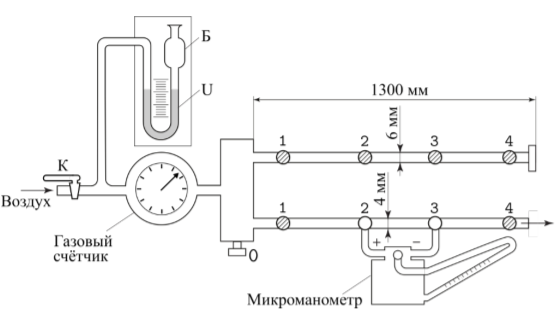
\includegraphics [scale=1]{photo 1.png}}
		\caption{Экспериментальная установка}
	\end{figure}
	
	\newpage
		
	\textbf{Результаты измерений и обработка данных:}
	\begin{enumerate}


		
	\item Запишем исходные данные: $d_1=4,10\pm 0,05$мм, $d_2=3,00\pm 0,1$мм, $d_3=5,20\pm 0,05$мм, погрешности: $\sigma_{\Delta V}=0,02$л,  $\sigma_{l}= 1$мм
	
	
	 \item Рассчитаем длину на которой поток можно считать  установившимся:
	 
	  $l_\text{уст1}=0,2R*Re=41,0\pm0,5$cм
	 
	$l_\text{уст2}=0,2R*Re=30\pm1$cм
	
	$l_\text{уст3}=0,2R*Re=52,0\pm0,5$cм
	\newpage
	
\item Измерим зависимости перепада давления $\Delta P$ на выбранном участке
	трубки от расхода газа Q для каждой трубки. Построим графики зависимости расхода от давления.
	
\begin{longtable}{|c|c|c|c|c|c|c|c|c|c|} \hline
	$N$ &  $\Delta V, \, \text{л}$  &   $l,\, \text{мм}$ &     $t_1, c$ &     $t_2, c$ &     $t_3, c$ &    $ Q, 10^{-3} \frac{\text{л}}{c} $ & $\Delta P, \, \text{Па}$\\ \hline
	1& 1.0   &  35 &  22,27 &  23,34 &  23,94 &    42,9 &   68,6\\ \hline
	2&   1.0 &  41 &  20,45 &  20,21 &  21,02 &    49,5 &   80,36\\ \hline
	3 &   1.0 &  56 &  16,25 &  16,92 &  16,60 &    60,9 &   109,76 \\ \hline
	4 &   1.0 &  60 &  15,88 &  15,78 &  15,79 &    63,2 &   117,6 \\ \hline
	5 &   1.0 &  69 &  14,06 &  14,68 &  14,34 &    69,9 &   135,24 \\ \hline
	6 &   1.0 &  74 &  13,46 &  13,93 &  13,32 &    74,0 &   145,04 \\ \hline
	7 &   1.0 &  79 &  13,15 &  12,94 &  13,12 &   76,3 &   154,84 \\\hline
	8 &   1.0 &  91 &  11,64 &  11,73 &  11,78 &    85,4 &   178,36 \\ \hline
	9 &   1.5 &  101 &  11,52 &  11,33 &  11,09 &    94,9 &   197,96 \\ \hline
	10 &  1.5 &  110 &  10,86 &  10,84 &  10,96 &    107,6 &  215,6 \\ \hline
	11 &  1.5 &  115 &  10,27 &  10,32 &  10,70 &    114,2 &  225,4 \\ \hline
	12 &  1.5 &  122 &  10,24 &  9,86 &  9,81 &  121,5 &  239,12 \\ \hline
	13 &  2.0 &  130 &  12,43 &  12,59 &  12,47 &    131,2 &  254,8 \\ \hline
	14&  2.0  &  140 & 11,95 &  11,58 &  12,42 &   146,6 &  274,4 \\ \hline
	\caption{ Данные для трубы d1}
\end{longtable}

\begin{figure}[H]
	\center{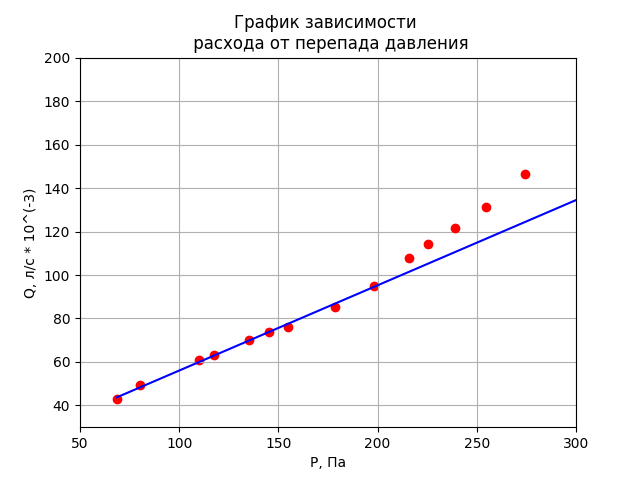
\includegraphics [scale=0.7]{graph 1.png}}
	\caption{}
\end{figure}


\item Коэффициент угла наклона графика: $k = (0,479 \pm 0,002)\cdot 10^{-6} \frac{\text{Па} \cdot c}{\text{м}^3}$

Искомая вязкость:
\[
\eta = \frac{\pi r^4 }{8 k l} = (18.6 \pm 0.7) \cdot 10^{-6} \text{Па} \cdot \text{c}
\]
По графику определим, когда ламинарный поток переходит в турбулентный:

 $Q \approx 100 \cdot 10^{-3} \frac{\text{л}}{c}$.
  Число Рейнольдса:$Re = \frac{Q \rho}{\pi r \eta} \approx 954 \pm 89$



		\begin{longtable}{|c|c|c|c|c|c|c|c|c|c|} \hline
		$N$ &  $\Delta V,  \text{л}$  &   $l, \text{мм}$ &     $t_1, c$ &     $t_2, c$ &     $t_3, c$ &    $ Q, 10^{-3} \frac{\text{л}}{c} $ & $\Delta P, \text{Па}$\\ \hline
		1& 0.5   &  25 &  15,16 &  15,14 &  15,64 &    32,6 &   49\\ \hline
		2&   0.5 &  35 &  12,27 &  12,27 &  12,00 &    41,3 &   68,6\\ \hline
		3 &   0.5 &  40 &  10,95 &  11,45 &  10,65 &    44,6 &   78,4 \\ \hline
		4 &   0.5 &  45 &  10,29 &  10,12 &  10,21 &    49,0 &   88,2 \\ \hline
		5 &  0.5 &  50 &  9,57 &  9,76 &  9,38 &    52,6 &   98 \\ \hline
		6 &   0.5 &  60 &  8,20 &  8,50 &  8,50 &   59,5 &   117,8 \\ \hline
		7 &   0.5 &  65 &  7,98 &  8,06 &  7,77 &   62,5 &   127,4 \\\hline
		8 &   1.0 &  75 &  14,32 &  14,50 &  14,87 &    68,9 &   147 \\ \hline
		9 &   1.0 &  85 &  13,76 &  13,33 &  13,62 &    74,0 &  166,6 \\ \hline
		10 &  1.0 &  90 &  12,81 &  13,15 &  13,05 &    77,2 &  176,4 \\ \hline
		11 &  1.0 &  95 &  12,46 & 12,51 &  12,98 &    78,7 &  186,2 \\ \hline
		12 &  1.0 &  100 &  12,19 &  12,4 &  12,24 &   82,9 &  196 \\ \hline
		13 &  1.0 &  105 &  12,38 &  11,92 &  11,85 &    88,3 &  205,8 \\ \hline
		14&  1.0  &  115 &  11,43 &  11,30 &  11,64 &   96,9 &  225,4 \\ \hline
		\caption{ Данные для трубы d2}
	\end{longtable}
	
	
	\begin{figure}[H]
		\center{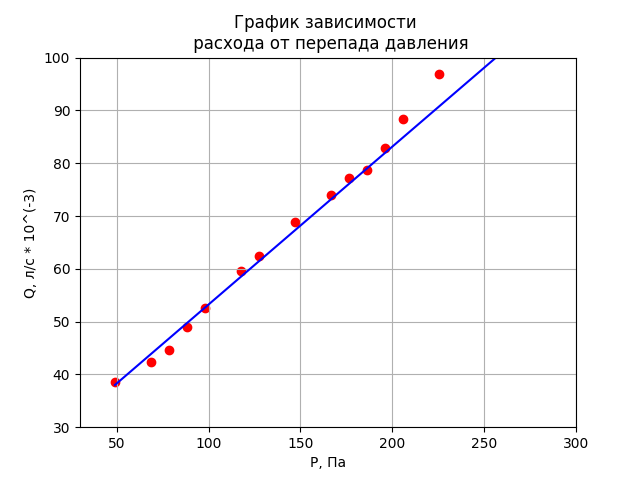
\includegraphics [scale=0.7]{graph 2.png}}
		\caption{}
	\end{figure}


	\item Коэффициент угла наклона графика: $k = (0,536 \pm 0,003)\cdot 10^{-6} \frac{\text{Па} \cdot c}{\text{м}^3}$
	
	Искомая вязкость:
	\[
	\eta = \frac{\pi r^4 }{8 k l} = (17.3 \pm 0.9) \cdot 10^{-6} \text{Па} \cdot \text{c}
	\]
	По графику определим, когда ламинарный поток переходит в турбулентный:
	
	$Q \approx 82 \cdot 10^{-3} \frac{\text{л}}{c}$.
	Число Рейнольдса:$Re = \frac{Q \rho}{\pi r \eta} \approx 1044 \pm 93$ 
	
	
	\newpage
		\begin{longtable}{|c|c|c|c|c|c|c|c|c|c|} \hline
		$N$ &  $\Delta V, \, \text{л}$  &   $l,\, \text{мм}$ &     $t_1, c$ &     $t_2, c$ &     $t_3, c$ &    $ Q, 10^{-3} \frac{\text{л}}{c} $ & $\Delta P, \, \text{Па}$\\ \hline
		1& 1.0   &  50 &  6,98 &  6,96 &  6,89 &    144,9 &   98\\ \hline
		2&   1.0 &  55 &  6,42 &  6,58 &  6,71 &    151,1 &  107,8\\ \hline
		3 &   1.0 &  60 &  6,17 &  6,18 &  6,32 &   161,2 &   117,6 \\ \hline
		4 &   1.0 &  70 &  5,78 &  5,89 &  5,79 &    172,4 &   137,2 \\ \hline
		5 &   1.0 &  80 &  5,27 &  5,40 &  5,25 &    188,6 &   156,8 \\ \hline
		6 &   1.0 &  90 &  5,21 &  5,07 & 5,05 &    196,0 &   176,4 \\ \hline
		7 &   1.0 &  100 &  4,76 &  4,79 &  4,59 &  210,3 &   196 \\\hline
		8 &   1.0 &  110&  4,66 & 4,60 &  4,55 &    217,3 &   216,6 \\ \hline
		9 &   1.5 &  115 &  6,55 &  6,86 &  6,48 &    227,2 &   225,4 \\ \hline
		10 &  1.5 &  120 &  6,52 &  6,29 &  6,56 &   234,3 &  235,2 \\ \hline
		11 &  1.5 &  125 &  6,48 &  6,11 &  6,49 &    241,9 &  245 \\ \hline
		12 &  1.5 &  130 &  6,11 &  6,34 &  6,20 &  245,9 &  254,8 \\ \hline
		13 &  1.5 &  135 &  6,18 &  6,07 &  6,04 &   250,0 &  264,6 \\ \hline
		14&  1.5  &  140 & 6,18 &  6,05 &  5,72 &    255,3 &  274,4 \\ \hline
		\caption{ Данные для трубы d3}
	\end{longtable}
	

	
	\begin{figure}[H]
		\center{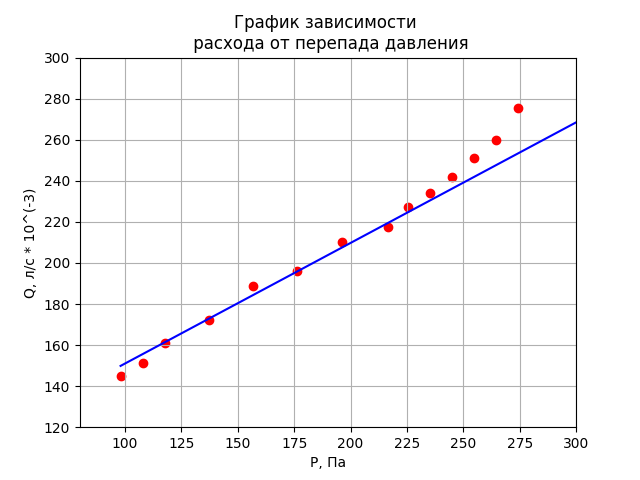
\includegraphics [scale=0.7]{graph 3.png}}
		\caption{}
	\end{figure}




\item Коэффициент угла наклона графика: $k = (1,112 \pm 0,005)\cdot 10^{-6} \frac{\text{Па} \cdot c}{\text{м}^3}$

Искомая вязкость:
\[
\eta = \frac{\pi r^4 }{8 k l} = (19 \pm 1) \cdot 10^{-6} \text{Па} \cdot \text{c} => \overline \eta = (18,3\pm 0,9)\cdot 10^{-6}  \text{Па} \cdot \text{c}
\]
По графику определим, когда ламинарный поток переходит в турбулентный:

$Q \approx 220 \cdot 10^{-3} \frac{\text{л}}{c} $.
Число Рейнольдса:$Re = \frac{Q \rho}{\pi r \eta} \approx 1769 \pm 88$ 
\newpage

\item Измерим перепады давления вдоль трубки d1, результат представим в виде графика и таблицы.


	\begin{longtable}{|c|c|c|}
		\hline 
		N & $\Delta P$, Па& L, см \\
		\hline
		1 & 166,6 & 10,5\\
		\hline
		2 & 176,4 & 30\\
		\hline
		3 & 192 & 40\\
		\hline
		4 & 245 & 50\\
		\hline
		5 & 318 & 70\\
		\hline
		6 & 467 & 90\\
		\hline
		7 & 633 & 120\\
		\hline
		8 & 702 & 130\\
		\hline
		\caption{Данные давления и расстояния}
	\end{longtable}
	
	\begin{figure}[H]
		\center{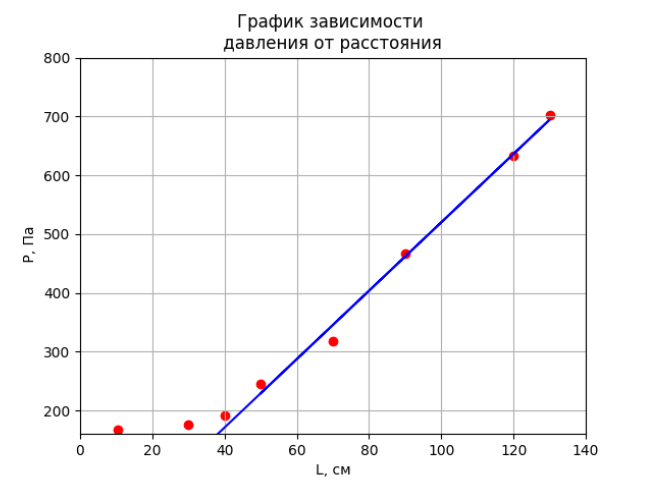
\includegraphics [scale=0.85]{graph 4.1.png}}
		\caption{}
	\end{figure}
	Таким образом получаем, что длина установления потока $l \approx 45$ см.
	
	Теоретическая оценка: 	$ l_\text{уст} = 0,2 R*Re = 42 \pm 3$см
	
	\item Измерим зависимость расхода от радиуса трубы при заданном градиенте
	давления. Построим график ln Q(ln R)
	
	
	\begin{longtable}{|c|c|c|c|c|}
		\hline 
		 & $\Delta V$, л & l, мм& $\Delta t$, с& $\Delta P$, Па\\
		\hline
		$d_1$ & 1 & 55&10,55&107,8\\
		\hline
		$d_2$ & 1 & 52&14,41&101,9\\
		\hline
		$d_3$ & 1 & 55&5,15&107,8\\
		\hline
		\caption{Данные давления и расстояния}
	\end{longtable}
	
	
	\begin{figure}[H]
		\center{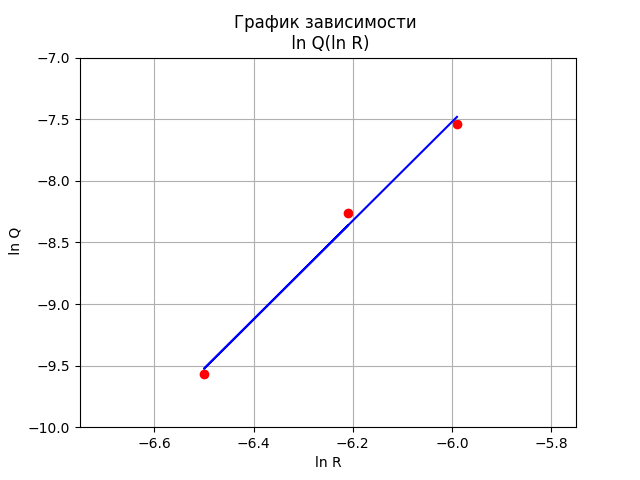
\includegraphics [scale=0.7]{graph 5.png}}
		\caption{}
	\end{figure}
	
	Таким образом мы получили наклон прямой $k=4,0\pm0,1$, что соответствует теоретической оценке.
	
	\textbf{Обсуждение результатов и вывод:}
	В данной работе мы экспериментально исследовали свойства течения газов по тонким трубкам	Измерили зависимости перепада давления $\Delta P$ на выбранном участке
	трубки от расхода газа Q. Измерили распределение давления газа вдоль трубки. Измерили зависимость расхода от радиуса трубы при заданном градиенте давления. По полученным данным построили графики и таблицы. Выявили область применимости закона Пуазейля и с его помощью определили коэффициент вязкости воздуха $\overline \eta = (18,3\pm 0,9)\cdot 10^{-6}  \text{Па} \cdot \text{c}$.

	
	
\end{enumerate}
\end{document}
